% !TeX root = ../main.tex

\chapter{电子回旋辐射与反常辐射}
\section*{引言}
本节首先阐明了电子回旋辐射成像诊断的基本原理,并提出了光学透镜表面优化的方案,为提升信噪比和后续实验研究奠定了理论基础。通过分析放电初期的电子回旋辐射信号,观测到具有前端峰值和台阶状特征的辐射结构。通过与国内外相关实验结果的对比,进一步探讨了反常多普勒效应的背景及其研究现状,为深入研究非热化电子演化过程提供了重要依据。
\section{电子回旋辐射成像诊断及光学优化}
\subsection{电子回旋辐射成像诊断简介}\label{sec:ECEI}
电子回旋辐射成像诊断\cite{RN1020}(Electron cyclotron emission imaging [ECEI] )是二维微波成像系统。ECEI大尺度光学透镜能够实现将像面中电子回旋辐射信号投射在物面天线上,实现对像面中温度波动测量。如\autoref{fig:ECEIstru}所示,图中左侧大矩形区域表示EAST装置D型截面,小矩形区域表示ECEI成像区间,红色光束表示接收光路,透镜的功能是实现变焦和场曲调节,使得接收天线能够有效探测到目标空间的辐射信号。天线负责接收等离子体中电子回旋辐射信号并对接收信号通过外差降频传输给后端中频系统,信号在中频经过降频滤波检波后得到的视频信号接入采集卡,通过模数转换变为数字信号,最后通过数据分析即可获得温度涨落分布时间演化图。ECEI具有大尺度高时间空间分辨率的观测优势,通过ECEI可以实现对大尺度MHD行为的直接观察,为研究磁重联过程中丰富的物理提供了有力的诊断工具。\autoref{fig:ECEIimag}展示的是Sawtooth\cite{RN1791}过程中观察到的温度涨落随时间的演化过程,相对于传统的一维电子回旋辐射诊断(ECE)\cite{RN742},ECEI诊断提供了更加丰富直观的物理图像。
\begin{figure}[ht]
  \centering
  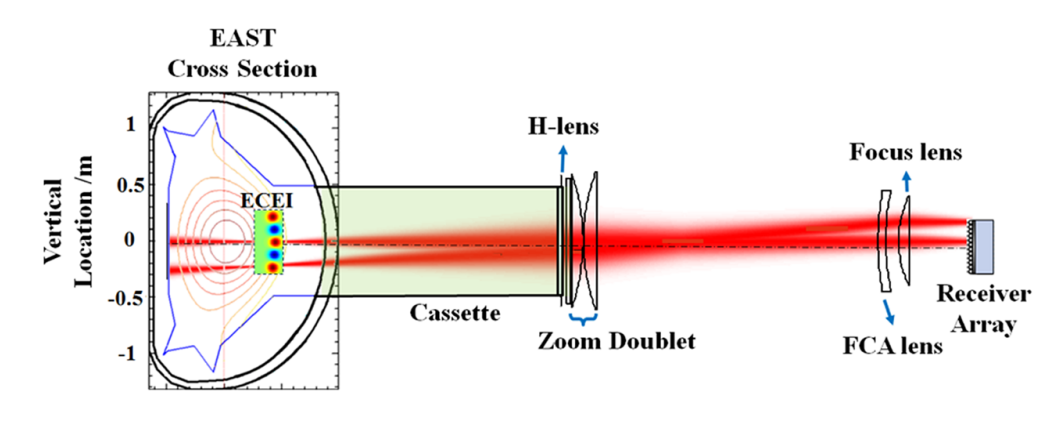
\includegraphics[width=12cm]{image9.png}
  \caption{\label{fig:ECEIstru} ECEI概念图\cite{RN1847},从左至右分别为EAST极向小截面(蓝色区域为ECEI观测范围)、接收透镜、ECEI天线阵列等 }
\end{figure}


\begin{figure}[h]
  \centering
  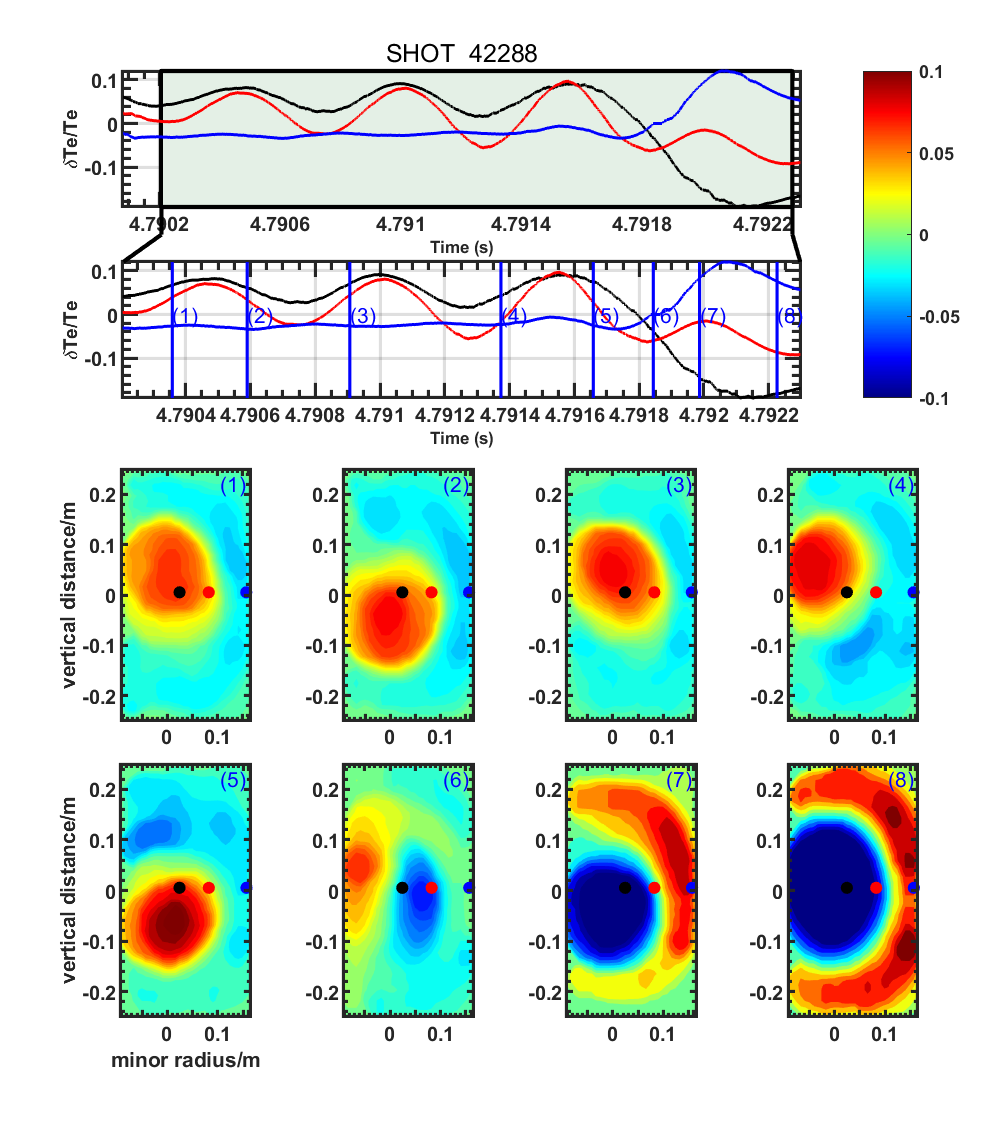
\includegraphics[width=14cm]{image10_1.eps}
  \caption{\label{fig:ECEIimag}EAST 装置中 ECEI 诊断观测到的锯齿破裂演化过程,不同颜色表示温度涨落分布,红色为正、蓝色为负,三条曲线对应矩形窗口中的三个空间位置}
\end{figure}

ECEI 诊断涉及到辐射频率与空间位置的对应关系,辐射强度与温度的对应关系。
\par \noindent
a.空间位置的对应关系
\par 根据经典电动力学知识,托卡马克中电子绕磁力线回旋运动会辐射出电磁波,由于电子回旋运动的非线性效应,电子回旋频率除了基频$f_{ce}$以外还存在该频率的高次谐波成分(\autoref{sec:A1}),因此电子回旋频率可表示为
\begin{equation}
nf_{ce}=n\frac{1}{2π}∙\frac{eB}{\gamma m_e} 
\end{equation}
其中n=1,2,3,…表示谐波次数,γ表示相对论修正因子,B表示托卡马克中纵场强度,B和大半径之间满足反比例关系:
\begin{equation}
B=\frac{B_0R_0}{R}
\end{equation}
这里$B_0$ 、$R_0$表示磁轴处磁场和大半径。由于纵场强度沿大半径方向单调递减(\autoref{fig:charac-f}),沿水平径向观测方向上,回旋频率和纵场强度满足一一对应关系,
\begin{figure}[ht]
  \centering
  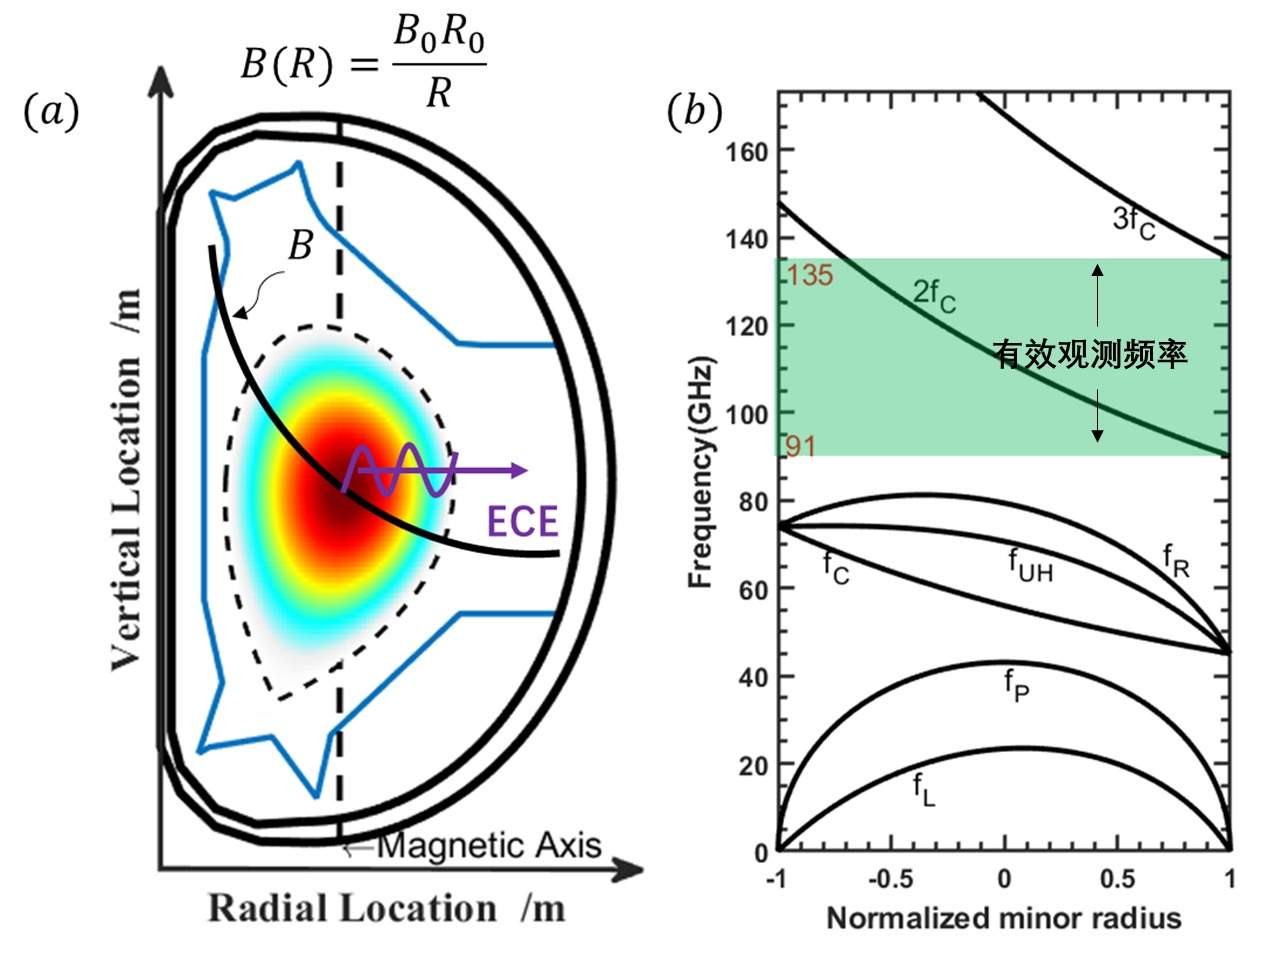
\includegraphics[width=12cm]{image11_2.png}
  \caption{\label{fig:charac-f} (a)托卡马克纵场分布图(b)EAST托卡马克装置下各特征频率分布图,图片为自绘}
\end{figure}
因此可以通过选择不同的频率实现对径向空间位置的分辨。
如\autoref{fig:charac-f}(b)所示,垂直于磁场的特征频率包括电子回旋频率$nf_c$、等离子体频率$f_p$,上杂化频率$f_{UH}$,左旋截止频率$f_{L}$以及右旋截止频率$f_R$等。垂直于磁场传播的电磁波主要存在两种偏振态,其中电场方向平行与磁场的波称为O波,电场方向垂直与磁场的波为X波。X波的截止频率和特征频率中的$f_R$相同,共振吸收频率为$f_{UH}$。O波的截止频率对应特征频率中的$f_p$。为了确保频率和空间位置的一一对应,用于接收的频率必须与其它频率没有重叠,同时该频率能从等离子体中传出来,不被共振或截止。综上所述,只有图中绿色阴影区间的$2f_c$的X波和$f_c$的O波可用于电子回旋辐射诊断,$2f_c$的O波因强度相对X波较弱而被舍弃。
\par 通过光学软件中射线追迹功能可获得ECEI不同极向天线对应的极向观测位置\cite{RN1367,RN1020},因此ECEI具有径向和极向空间分辨能力的二维空间诊断。
\par \noindent
b.辐射强度与温度的对应关系 \par
电子回旋辐射在等离子体区域的输运主要由发射和吸收两个过程决定。在介电常数近似为1的稀薄等离子体中$(ω_{pe}\ll ω$,等离子体频率远小于电磁波频率),辐射输运方程可表示为\cite{RN1414}
\begin{equation}
\frac{\dif  I(\omega)}{\dif s}=\eta(\omega)-\alpha(\omega) I(\omega)
\end{equation}
这里s表示辐射路径,$I(\omega)$表示单位面积单位立体角单位角频率的辐射功率,$\eta(\omega)$表示发射率,$\alpha(\omega)$表示吸收系数,从路径位置$s_1$到$s_2$过程中,该方程的解为:
\begin{equation}\label{eq:optical_s}
I\left(s_{2}\right)=I\left(s_{1}\right) e^{-\tau}+\frac{\eta}{a}\left[1-e^{-\tau}\right]
\end{equation}
其中光学厚度$\tau$的定义是
\begin{equation}
\tau=\int\limits_{s_1}^{s_2}\alpha(\omega)\dif s
\end{equation}
当光学厚度$\tau\gg1$时有
\begin{equation}\label{eq:Is2}
I(s_2)=\frac{\eta}{\alpha}
\end{equation}
此时辐射满足黑体辐射。根据黑体辐射定律,单位路径等离子体发射功率等于其吸收的功率,即$\eta+\alpha B(\omega)=0$,且黑体辐射表面亮度为:
\begin{equation}\label{eq:Itik}
B(\omega)=\frac{\eta}{\alpha}=\frac{\hbar \omega^{3}}{8 \pi^{3} c^{2}} \frac{1}{\exp \left(\frac{\hbar \omega}{T}\right)-1}
\end{equation}
这里考虑的是线极化辐射,所以和课本中黑体辐射公式相差1/2 ,在低频区域$\hbar \omega \ll T$时,我们得到Rayleigh-Jeans公式
\begin{equation}\label{eq:blk}
B(\omega)=\frac{\omega^2T}{8\pi^3c^2}
\end{equation}
结合\autoref{eq:Is2}式和\autoref{eq:blk}式得:
\begin{equation}\label{eq:Te-to-I}
T_e(R(\omega))=\frac{8\pi^3c^2}{\omega^2}I(\omega)
\end{equation}
此时不难看出辐射强度$I(\omega)$与温度$T_e(R)$满足线性关系,原则上通过测量辐射强度结合温度\autoref{eq:Te-to-I}我们就可以准确获得温度。系统对信号强度I的响应通常满足线性关系,即$I_{measure}=k I$,实际上精确测量比例系数k是比较困难的,通常需要借助TS诊断或相关等离子体中的物理过程\cite{RN1381}。目前ECEI信号的主流分析手段是通过测量信号$I_{measure}$的涨落来分析温度的相对涨落,即
\begin{equation}
\frac{\delta T_e}{T_e}=\frac{\delta I_{measure}}{I_{measure}}
\end{equation}
当光学厚度小于1时对应光学薄,对\autoref{eq:optical_s}右侧第二项一阶泰勒展开可得
\begin{equation}\label{eq:optical_s2}
I\left(s_{2}\right)=I\left(s_{1}\right) +\frac{\eta}{a}\tau \approx I\left(s_{1}\right)+ \eta \Delta s
\end{equation}
其中$I(s_1)$表示的是边界反射信号,不考虑反射则为0。此时辐射强度主要取决于发射率$\eta$的形式。如\autoref{fig:etamax}是根据2X波电子回旋辐射方程\eqref{eq:Xradiation}所绘,在固定电子速度条件下电子回旋辐射强度主要由垂直方向电子速度贡献,强烈依赖于
电子垂直方向速度。
\begin{figure}[ht]
  \centering
  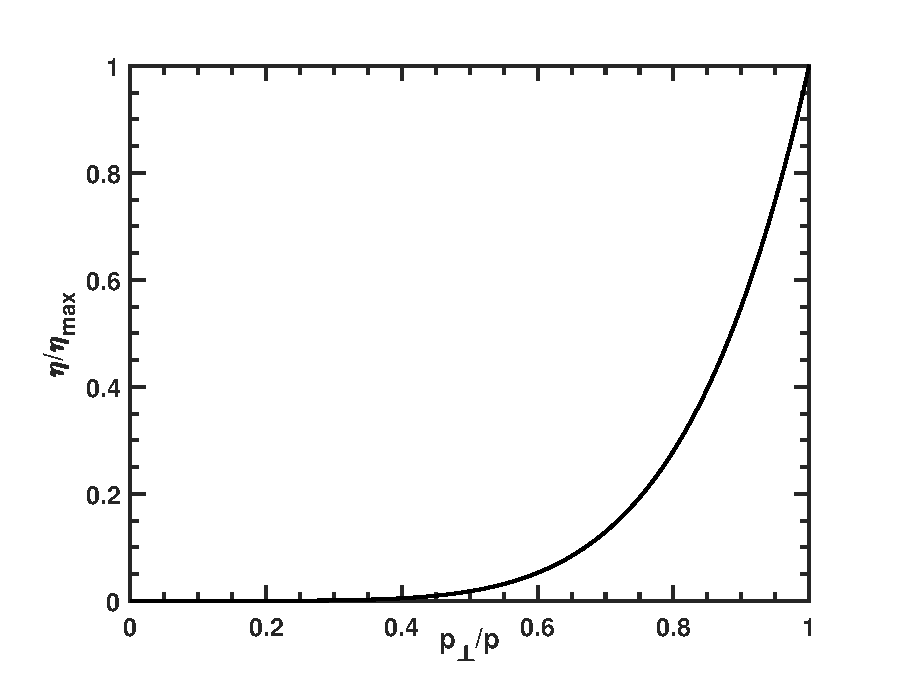
\includegraphics[width=12cm]{etadivideetamax.eps}
  \caption{\label{fig:etamax} 垂直磁场方向传播的2X波辐射强度与电子运动角度之间的关系}
\end{figure}
因此光学薄时电子回旋强度的变化主要反映垂直方向电
子速度的变化。在放电初期或低密度放电过程中,光学厚度一般都小于一,电子
速度分布中非热化分布的电子会产生丰富的辐射现象,通过合适的物理模型解释
辐射现象便是本文研究的主要目的。

%\vspace*{2em}
由于EAST装置大窗口资源有限,ECEI系统处于低杂波系统和NBI系统之间且与NBI系统共D窗口,空间十分狭小。目前中国科大正在致力于合并ECEI和MIR(Microwave Imaging  
Reflectometry)光路。合并光路使科大微波成像诊断系统更加紧凑,适应当下
的空间条件。同时通过ECEI和MIR联合诊断可以实现对托卡马克等离子体同一区域
密度和温度波动同时测
量,对研究边界局域模(ELM)、微撕裂模(MTM)等都具有重要的意义。
MIR利用大尺度透镜通过收集等离子体截止层处反射的微波信号,实现对
托卡马克截止层密度波动成像\cite{mazzucato2001microwave}。如\autoref{fig:MIR}所示,MIR的微波为系统主动
发射的多频率信号,通过照明光路对微波波前曲率调节实现和等离子体截止层曲率
匹配,这样反射的微波信号才能避免多普勒效应对相位的影响,同时实现最大反
射信号强度,提高成像质量。反射信号经过接收光路投影在天线位置,通过天线
上二极管混频降频后进入中频系统实现对微波信号IQ鉴相,获得相位波动信息。
不同极向位置的天线对应不同极向位置的截止层位置,不同频率的微波信号对应
不同截止层的径向位置,通过这种二维探测阵列实现对密度波动的二维成像。
\begin{figure}[ht]
\centering
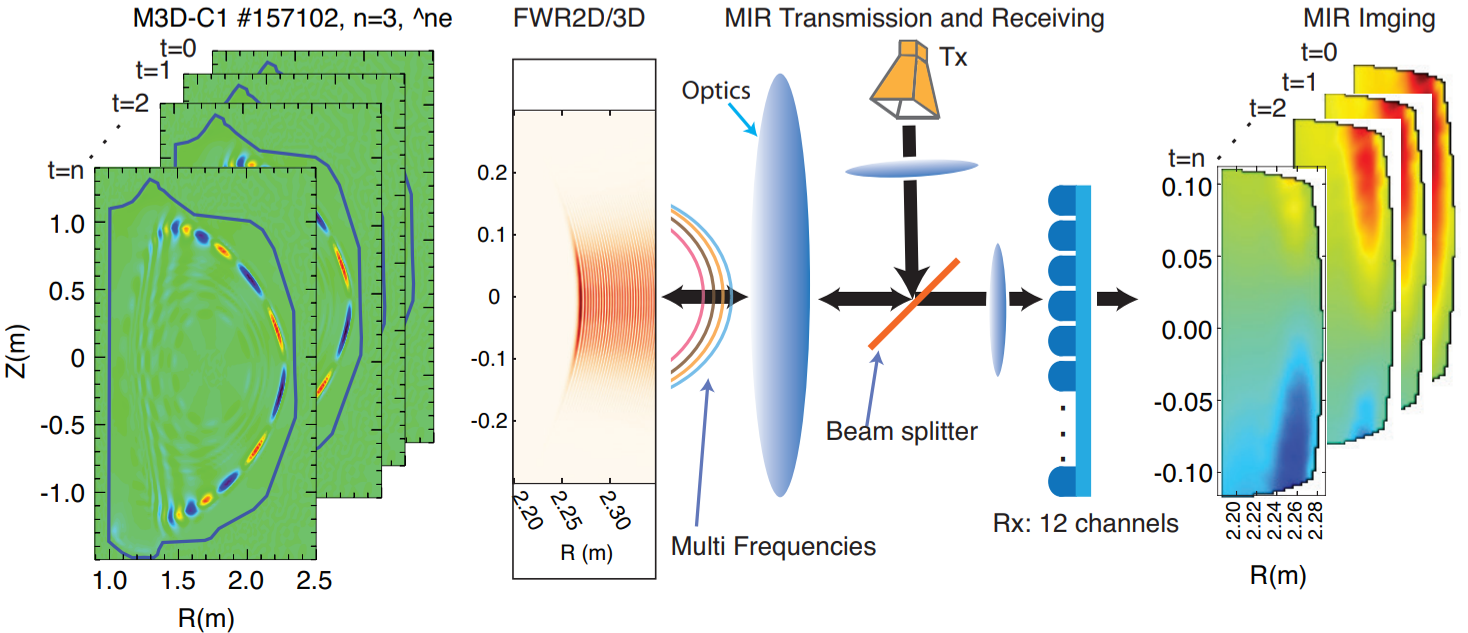
\includegraphics[width=15cm]{image12.png}
\caption{\label{fig:MIR}MIR数值合成诊断图,图片来源自
X.Ren\&M.Chen\cite{RN1190},其中M3D-C1为磁流体程序,用来模拟产生边界
谐频模(EHO),FWR为全波解程序,用来模拟微波在等离子体中的传播。微波
通过照明光路进入等离子体“照亮”截止层,携带截止层相位变化信息的微波经大尺度透镜投影在接收天线被天线收集,经中频系统检波分析获得最终的密度波动成像图}
\end{figure}
\par 
大尺度透镜不论在ECEI还是MIR系统中都承担着重要作用,通过多个透镜的组合
可以实现对波前曲率、场曲、聚焦位置、景深等光学参数调节。然而事物的发展
总是具有两面性,透镜组同时会导致微波信号在经过多组透镜时的反射损失增
加。当两套系统合并光路后,原本微弱的辐射的信号还需要进一步一分为二分别
进入两套系统,使得信号弥加珍贵。为了减小信号损失必须要采取相应的手段优
化透镜,降低微波信号在透镜表面的反射损失。其中槽纹表面结构作为广泛应用于可见光学波段增透的技术手段\cite{savin2015black},我们尝试在微波波段同样采用槽纹结构解决透镜表面反射损失问题。
\subsection{大口径高斯光学成像透镜的表面优化}
针对合并光路,减少微波损失的途径主要有三种:1.减小透镜表面反射;2.减小透镜介质损耗正切角对微波的耗散;3.减小分光过程中必要的信号损失。我们选取高密度聚乙烯材料作为光学透镜,高密度聚乙烯材料损耗正切角仅为0.00004-0.001,100Ghz的微波信号单位路径长度损失约为$20\%$,是目前作为微波透镜优质材料。对于第三种方案,由于ECEI和MIR共光路,我们采用罗杰斯分束片将微波信号均分为二分别进入ECEI系统和MIR系统,这样的不足之处是会损失一半有效微波信号。另一种取代罗杰斯分束片的方法是使用频率选择表面(FSS)。由于ECEI和MIR不共频段,原则上可以利用FSS实现选择性分光,使得MIR频率段透射(或反射)进入MIR系统,ECEI信号反射(或透射)进入ECEI系统,实现无损分光。但最后的测试结果并不理想,FSS结构依然有待改进。因此最终可优化的就是第一种:减小透镜表面反射。
\par 透镜表面一般优化方法是贴增透膜,单层增透膜广泛用于可见光波段,通过干涉相消的方法抑制反射波,由于其结构特征只能实现特定频率的波长增透。为了实现宽频增透效果,人们提出了多层膜结构\cite{RN2059}。多层膜结构虽然能实现宽频增透,但是对材料、镀膜精度要求苛刻。对于毫米波透镜,其膜层厚度也需要在毫米量级,在实际操作透镜时难免会因为碰触导致镀膜层破损。大自然里的夜行动物早就进化出了广谱(或者说适应宽波长范围)光学增透结构进而提高夜间视力。20世纪末,人们通过电子显微镜对夜间动物的角膜观测发现在夜间动物的眼角膜上均匀分布高度和距离约200nm的角锥结构\cite{RN693},经研究发现该结构可以有效提高空气和角膜之间,波长在400-700nm之间光的透射率,因此这种表面也称为抗反射结构表面(ARS, Anti-Reflection Structure)。夜间动物的眼睛(如飞蛾)之所以有敏锐的视力,除了视觉感光系统灵敏,大自然在其眼角膜上赋予的角锥结构也使得其具有更加优异的光学利用率,光线可以几乎无损的从空气进入眼角膜内,然后被接收分析处理。目前抗反射结构表面多用于可见光波段,而在微波频段下的应用甚少,微波成像诊断系统主要工作在W波段和F波段,拥有复杂的光学系统,微波在透镜表面的反射会降低信噪比或导致透镜之间的驻波效应。为简化物理模型,我们这里考虑一维槽纹结构作为ARS表面,定量研究它的微波增透效果。\par
如\autoref{fig:1dg}(a)所示,我们以一维槽纹结构为例,把槽纹结构从顶端到底端分割成多个小区间(\autoref{fig:1dg}(b)),在每个区间可以认为是折射率为n的等效介质层(\autoref{fig:1dg}(c)),这样的缓变介质层使得微波能够无反射地从空气传播到介质,因为根据Fresnel反射定律,只有入射层和折射层折射率不一致时才存在反射电场,而在缓变介质层中,由于z处折射率和z+dz(dz→0)处折射率增量dn→0,在任何位置反射率几乎都为零,因此微波能无反射损失从空气进入介质中。以上为ABS表面的增透原理,具体定量分析如下:\par
当电磁波入射在槽纹结构表面时,为了避免高阶衍射对能量的损耗只保留零级衍射,根据光栅方程$2π/λ*(sinθ_i±sinθ_m )=2πm/Λ$,当 m<1时槽纹周期Λ和微波波长$λ$之间需要满足$Λ<λ/(n_s+n_i )$,其中$n_s$表示介质折射率,$n_i$表示入射空间折射率。该不等式能保证电磁波以任何角度入射都只存在零级衍射。根据二阶等效介质理论(EMT, Effective Medium Theory)\cite{RN694},在等效多层矩形堆栈结构中每一层等效折射率大小为:
\begin{figure}[ht]
\centering
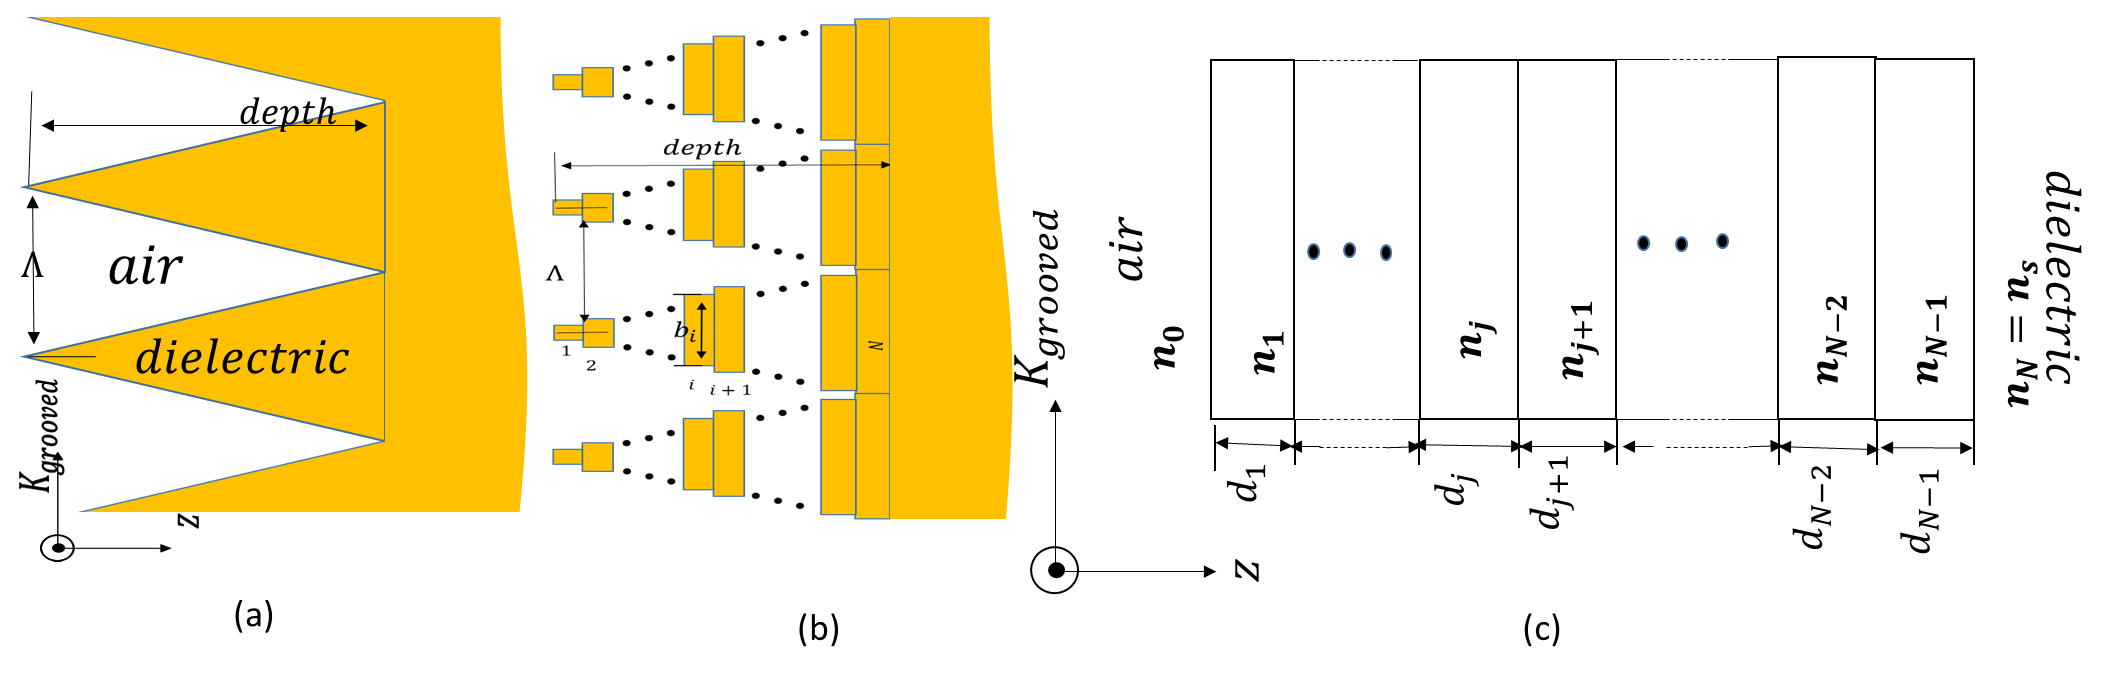
\includegraphics[width=14cm]{image13.png}
\caption{\label{fig:1dg} (a)一维槽纹结构表面,其中黄色部分为介质。(b)将三角结构等效为多层矩形结构堆栈。(c)将多层结构等效为折射率不同的介质堆栈}
\end{figure}
\begin{subequations}
\begin{align}
&\epsilon_{E \perp K}^{(2)}(z)=\epsilon_{E \perp K}^{(0)}(z) {\left[1+\left(\frac{\Lambda}{\lambda}\right)^{2} \frac{\pi^{2} }{3} f(z)^{2}(1-f(z))^{2} \frac{\left(\epsilon_{s}-\epsilon_{i}\right)^{2}}{\epsilon_{0}\epsilon_{E \perp K}^{(0)}(z)}\right] } \\
&\epsilon_{E \perp K}^{(0)}(z)  =f(z) * \epsilon_{s}+(1-f(z)) * \epsilon_{i}
\end{align}
\end{subequations}
$ϵ_s$与$ϵ_i$分别表示介质和入射空间介电系数,$f(z)$为$z$处槽纹结构的占空比。当$z=d$时($d$表示槽纹高度),$f(d)=1$;$z=0$时,$f(0)=0$。$\epsilon_{E\perp K}^2 (d)=\epsilon_s$,$\epsilon_{E\perp K}^2 (0)=ϵ_i$。$E⊥K$表示电场偏振方向和槽纹波矢方向垂直,$E\parallel	K$的情况可参考Daniel H. Raguin \&G. Michael Morris\cite{RN694}。 电磁波电场在j层及j层以内的总反射率为:
\begin{equation}\label{eq:iteration}
\rho_{\mathrm{j}}=\frac{\mathrm{r}_{\mathrm{j}}+\rho_{\mathrm{j}+1} \exp \left(2 \mathrm{i} \delta_{\mathrm{j}+1}\right)}{1+\mathrm{r}_{\mathrm{j}} \rho_{\mathrm{j}+1} \exp \left(2 \mathrm{i} \delta_{\mathrm{j}+1}\right)}
\end{equation}
其中$r_j$表示j和j+1层之间电场的反射率,$δ_j$表示$(2πn_j d_j)/λ  cos⁡(θ_j )$,$n_j$为j层等效折射率,$i=\sqrt{-1}$,$ρ_0$表示槽纹表面总反射率。最终槽纹表面反射率可以通过方程\autoref{eq:iteration}代算出。
\par HDPE材料具有低损耗正切角,可塑性强,被广泛用于微波透镜材料。这里以HDPE材料为例,取$ϵ_s=2.78$,研究不同尺寸的1D三角槽纹对透射率的影响。首先考虑这样一种状态:平面电磁波从空气正入射至无限大介质过程的反射率,其中空气和介质的交界面为无限大平面。利用EMT方法,取三角槽纹表面,槽纹厚度为d,周期为$Λ$,取入射电磁波频率为$87.5GHz$。槽纹结构从顶端到介质等效介电如\autoref{fig:efec}(a)图所示,槽纹结构实现了从空气到介质之间介电常数的缓慢增长。如\autoref{fig:efec}(b)所示,反射率随槽纹厚度d的增加迅速减小,当槽纹厚度达到两倍波长时反射率将减少至不到0.1\% 。ABS表面显著之处在于它不同于增透膜通过干涉的方法实现增透,在理论上这种结构能够实现对满足$λ>Λ(n_s+n_i )$所有频率实现增透,它的最小截止波长为$λ_c=Λ(n_s+n_i )$,这是根据零级衍射条件得到的。
\begin{figure}[ht]
\centering
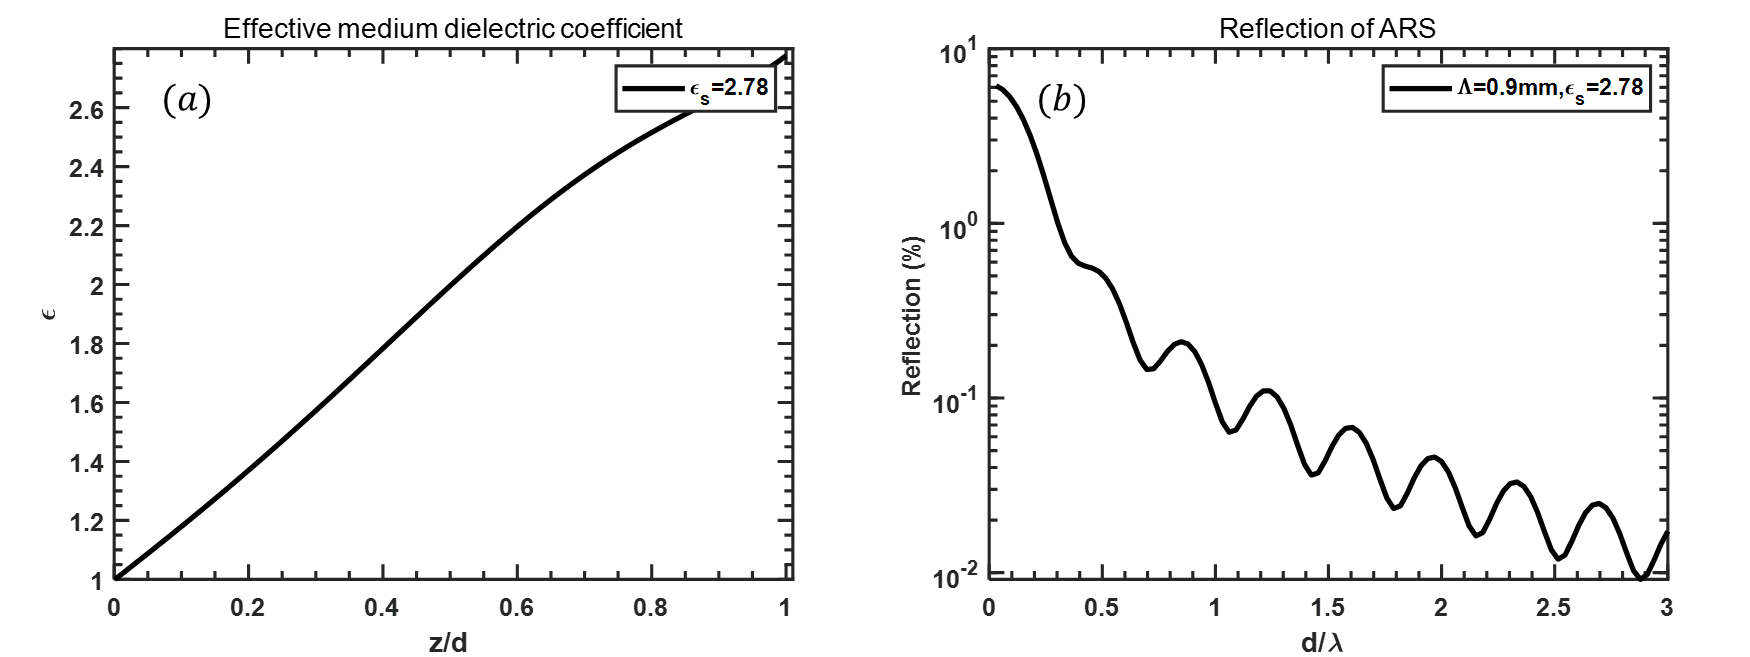
\includegraphics[width=14cm]{image14.png}
\caption{\label{fig:efec}(a)从空气到介质等效介电常数分布。(b)反射率随三角槽纹厚度的变化关系}
\end{figure}
\begin{figure}[ht]
\centering
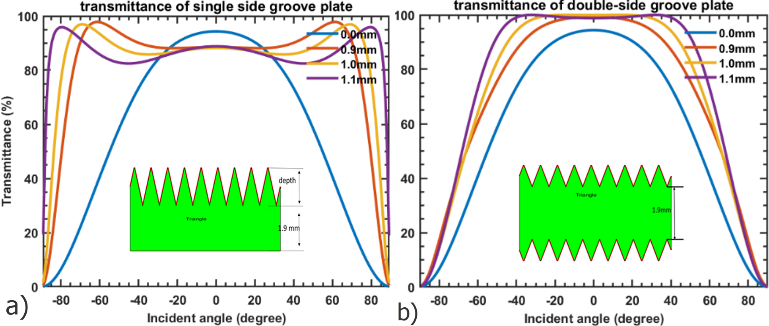
\includegraphics[width=14cm]{image15.png}
\caption{\label{fig:Ta}不同刻槽深度与入射角下单面槽纹板和双面槽纹板透射率,计算中将槽纹结构划分为1000个等效介质层}
\end{figure}
\begin{figure}[ht]
\centering
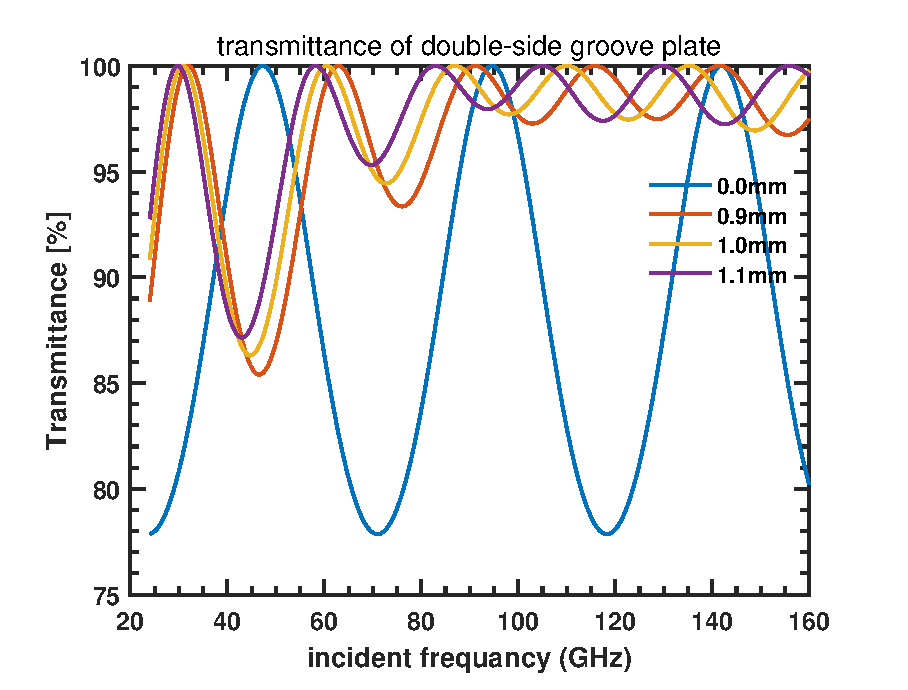
\includegraphics[width=12cm]{Transmittance_Freq.eps}
\caption{\label{fig:Trans_Freq}双面槽纹板不同刻槽深度下垂直入射电磁波透射率与频率变化关系}

\end{figure}
\begin{figure}[ht]
\centering
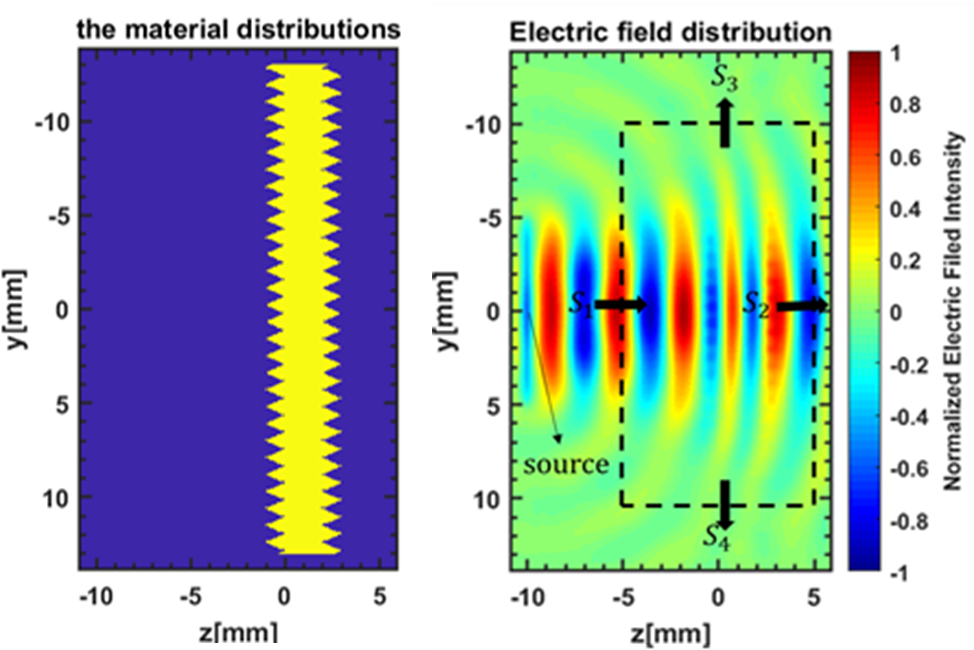
\includegraphics[width=12cm]{image16.png}
\caption{\label{fig:Na}双面一维三角槽纹结构模型以及FDTD计算过程中电场强度分布}
\end{figure}


\par
以上分析只考虑了空气-介质界面反射率的计算,在实际透镜中,我们需要考虑整个电磁波传播经过透镜后的透射率大小,为了方便计算,这里选择透镜形状为平板结构。如\autoref{fig:Ta}所示,平板厚度为1.9mm,频率87.5Ghz,固定槽纹周期$Λ=0.9mm$。如\autoref{fig:Ta}(a)展示了不同刻槽深度下单面槽纹透射率随角度的变化关系。从图中可看出单面槽纹正入射透射率甚至低于无槽纹的平板结构,且单面槽纹透射率随入射角存在两边凸中间凹的趋势,对增透的效果并不理想。反观双面槽纹具有大角度区域的增透效果,且刻槽深度越深,实现增透的角度区间越大。\autoref{fig:Trans_Freq}展示了不同刻槽深度下双面槽纹正入射电磁波透射率和频率的变化关系。对于刻槽深度大于0.9mm的双面槽纹板在频率为60GHZ-160GHZ透区间射率从最低77\%提升到到97\%以上,实现了宽频广角增透效果。我们通过时域有限差分 (Finite Difference Time Domain,FDTD)进一步模拟了双面槽纹电磁波传播过程,并根据能流计算了其对应的透射率。如\autoref{fig:Na}及\autoref{table:Comp},FDTD与EMT得到的结果几乎一致\cite{RN2060}。

\begin{table*}[h]
  \centering
  \caption{\label{table:Comp}FDTD与EMT计算结果对比}
  \label{tab:exampletable}
  \begin{tabular}{lcccccc}
    \toprule
   \multirow{2}{*}{类型}  & \multirow{2}{*}{$S_1$} & \multirow{2}{*}{$S_2$}  &  \multirow{2}{*}{$S_3$}  & \multirow{2}{*}{$S_4$}    &\multicolumn{2}{c}{透射率}
   \\

{}&{}&{}&{}&{}&FDTD&EMT\\

    \midrule
    空气 &342.9&338.3&0.26&-0.29&100\%&100 \\
    平板 & 318.9 &315.8&0.01&-0.01&93.3\%&93.6\%  \\
    单面槽纹 & 303.9 &303.5&0.22&-0.26&89.7\%&89.69   \\
双面槽纹   &338.5&337.4&0.01&0.01&99.72\%&99.17\%\\
    \bottomrule
  \end{tabular}
  \note{注:$S_i$表示第i个面的能流}
\end{table*}

在实验验证过程中,由于HDPE 材料无法通过有效的手段加工出符和要求的槽纹结构,目前只能3D打印制作符合要求的槽纹表面。而打印所用材料ABS (介电常数约2.8\cite{RN2062})其损耗正切角约是HDPE的10倍\cite{RN2061},信号在介质中的损失无法准确评估,透射率测量的实验只能定性分析透射率形状是否和理论一致。如\autoref{fig:exp}(a), 加工的单面槽纹板槽纹周期为0.9mm,高度为1.1mm,板厚约为1.9mm。\autoref{fig:exp}(b)为测量平台示意图,将透镜放在发射源一倍焦距处以构造准平行光,使电磁波入射角方向基本保持一致,最后再通过透镜在一倍焦距处收集透射电磁波。透镜轴线方向相对与测量轴线方向有一定偏角,以避免驻波效应对测量结果的影响,待测平板置于两透镜之间。测量结果如\autoref{fig:expdata}所示,单侧槽纹透射率与模拟结果出现相同的变化趋势,其中右侧有一个点为测量误差导致透射率出现严重偏离。



\begin{figure}[ht]
\centering
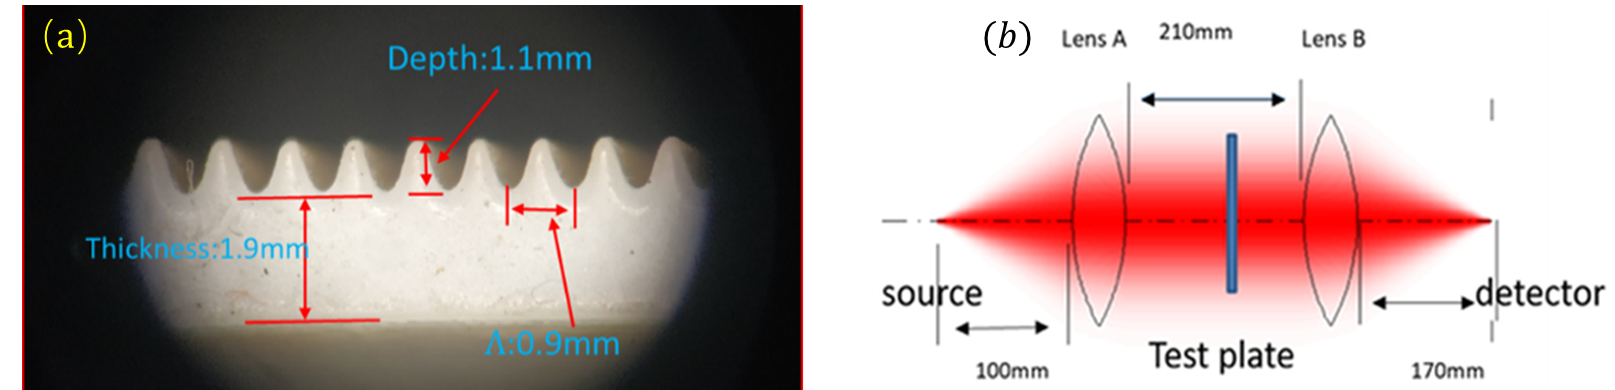
\includegraphics[width=14cm]{image17.png}
\caption{\label{fig:exp}(a)3D打印的单侧槽纹平板(b)透射率测量示意图}
\end{figure}

\begin{figure}[ht]
\centering
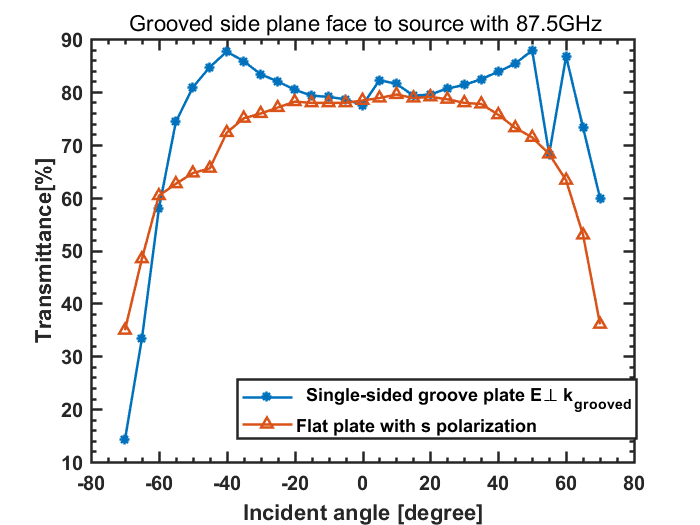
\includegraphics[width=14cm]{image18.png}
\caption{\label{fig:expdata}单侧槽纹板和平板在不同角度下透射率的变化}
\end{figure}

根据理论计算,在 HDPE 材料表面刻蚀周期为 0.9 mm、槽深为 1.1 mm 的一维三角槽纹结构,可将厚度为 1 mm 的平板在 40 GHz–160 GHz 微波正入射条件下的最低透射率由 77 \% 提高至 98 \%以上。该优化设计方案将有助于显著提升电子回旋辐射成像诊断的信噪比,改善成像质量,并为反常电子回旋辐射现象(如反常多普勒效应)的观测提供更加可靠的数据支撑。

%\clearpage
\section{电流爬升期电子回旋辐射}
    本节展示了在 EAST 装置第 64987 次放电(即第 64987 炮)中,ECEI 对反常辐射现象的实验观测结果。 如 \autoref{fig:eceregion} 所示,蓝色矩形区域表示 384 道 ECEI 的观测范围;蓝色虚线为通过 EFIT 反演得到的最后闭合磁面;红色长条则对应 32 道 ECE 的观测位置。 \autoref{fig:eceregion}(b) 中,Vloop 表示放电环电压,Ip 表示等离子体电流,$<n_e>$表示电子弦平均密度,HX 表示硬 X 射线谱强度,SXR 表示软 X 射线强度,ECE 表示电子回旋辐射信号。从 \autoref{fig:eceregion}(b) 可见,放电初期
\begin{figure}[ht]
\centering
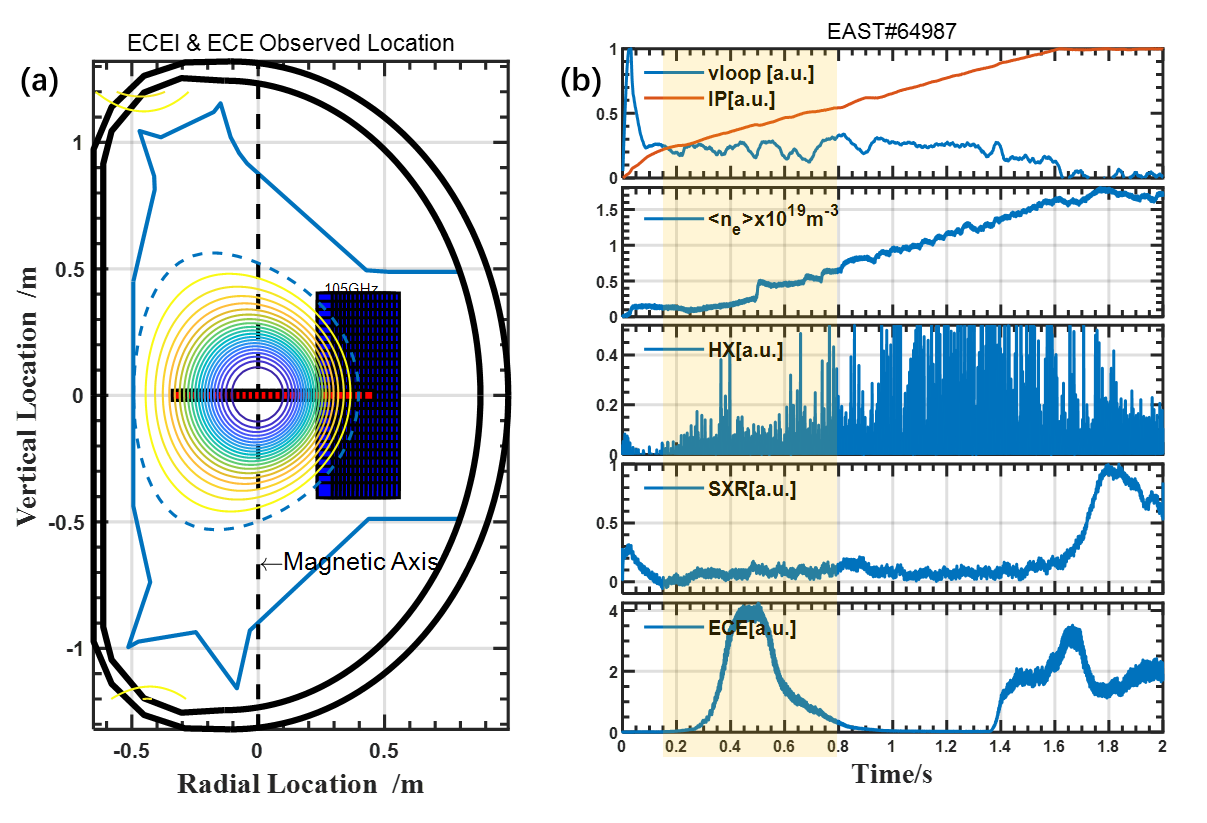
\includegraphics[width=14cm]{image96_2.png}
\caption{\label{fig:eceregion}(a)ECEI观测区域示意图 (b)EAST放电参数图,Vloop表示放电环电压,Ip表示等离子体电流,$<n_e>$表示电子弦平均密度,HX表示硬X射线谱强度,SXR表示软X射线强度,ECE表示电子回旋辐射信号}
\end{figure}
\begin{figure}[ht]
\centering
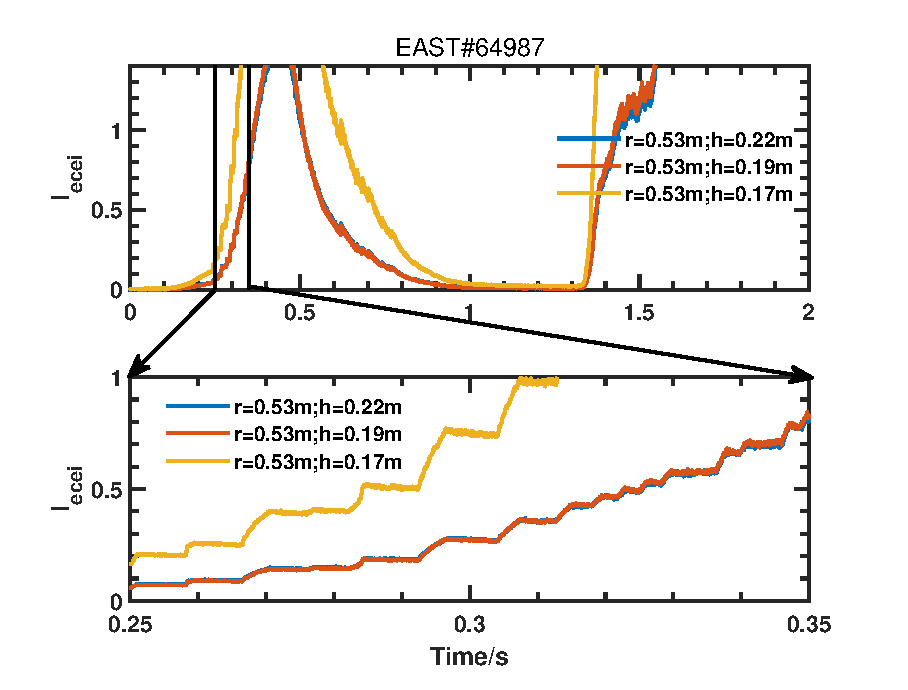
\includegraphics[width=14cm]{image20_1.eps}
\caption{\label{fig:ecestep}电子回旋辐射中的台阶结构,其中$I_{ecei}$表示测量得到的辐射强度,(r,h)表示三道信号所在托卡马克极向剖面空间位置,r表示托卡马克小半径位置,h表示高度}
\end{figure}
环电压Vloop迅速上升紧接着下降,EAST装置 通过消耗欧姆储能产生等离子体,欧姆加热开始驱动等离子体电流爬升,电子密度出现小幅度上升并在之后的0.5s内维持在约$0.2\times10^{19}/m^3$平台。与此同时,从\autoref{fig:eceregion}(b)可看出在0.5s时间SXR和HX无明显变化,说明此时还未产生高能电子,但是电子回旋辐射信号在约0.2s后迅速抬升并在约0.5s达到顶峰,之后缓慢下降,针对该回旋辐射变化的物理机制本文将在\autoref{sec:startup}展开探究。如\autoref{fig:ecestep}所示,为了观察电子回旋辐射信号更多细节特征,我们将ECE信号其中一段时间展开,此时发现了一种显著的现象:在辐射信号抬升的过程中存在一个一个step结构。后来发现,这种类似量子跃迁的现象早在上世纪70年代就已经在实验上发现\cite{RN725}。\par
1976年, D.A.Boyd\cite{RN725}在ATC托卡马克装置上通过测量沿装置大半经方向的电子回旋辐射强度,首次发现了辐射过程出现的step结构。如\autoref{fig:DAB}所示,其中上图表示频率在38GHz-110GHz区间的辐射强度,辐射迅速上升时(上升时间<10μs)伴随着环电压信号的迅速上升,D.A.Boyd将这种现象解释为在出现正电压峰时电子速度空间出现了快速角度散射,导致回旋辐射迅速上升。我认为D.A.Boyd是基于这样一种朴素的物理图像提出了这种猜想:首先系统的环电压与逃逸电子有关,环电压出现正电压峰时说明逃逸电子突然出现阻尼或损失,当逃逸电子出现了快速角度散射时相当于增加了逃逸电子的阻尼。同时被散射的逃逸电子垂直能量增加,因此该过程会导致回旋辐射增加和环电压上升。然而D.A.Boyd对逃逸电子被散射的具体原因并没有给出解释,1979年H. Knoepfel将D.A.Boyd观测到的step现象归因于ADE\cite{RN1030}。时至今日,关于这种现象的讨论已经持续了近50年\cite{RN1863,RN964,RN786,RN1866,RN1554,RN2102,RN1868,RN975,RN1859,RN798},普遍认为产生的原因是ADE。
\begin{figure}[H]
\centering
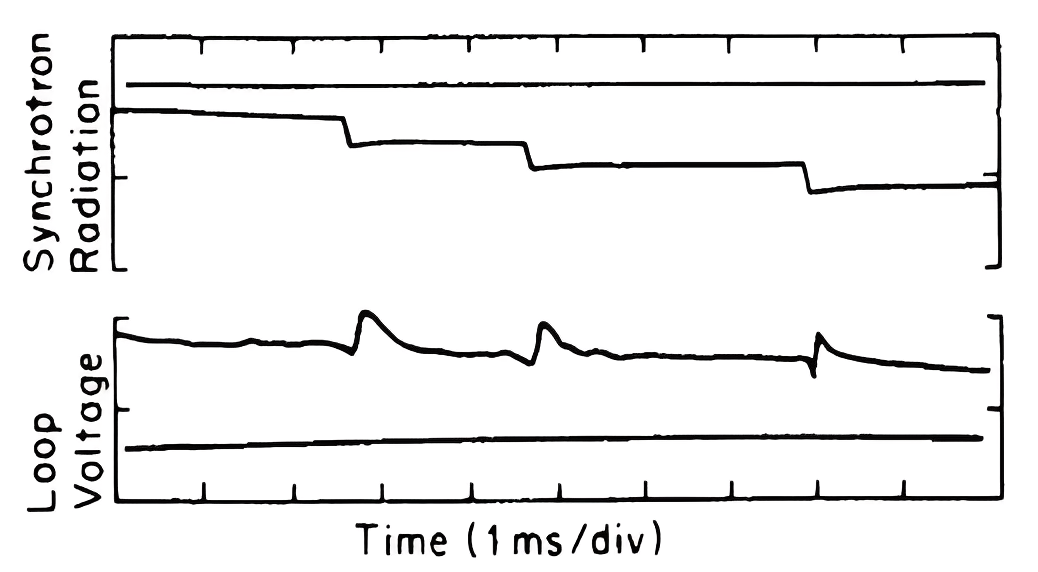
\includegraphics[width=12cm]{image25_1.png}
\caption{\label{fig:DAB}辐射强度‘跃迁’和环电压正电压尖峰出现时间一致,上图轨迹线表示辐射强度,辐射频率以$2ω_{ce}$占主导,下图表示环电压变化(5V/div),水平参考直线表示辐射本底和电压本底}
\end{figure}
\par 因此,可以认为本节所观测到的辐射 step 结构与早期实验中的结果具有较高的一致性,其出现时间与环电压的正电压峰高度相关,说明该现象很可能与等离子体启动阶段逃逸电子的角度散射过程密切相关。结合后续章节中对反常多普勒效应的理论分析与数值模拟,我们将进一步探讨这种辐射增强的物理机制,并尝试从速度空间动力学的角度揭示 step 结构的形成条件及其辐射与逃逸电子分布的关系。





\section{小结}
本章介绍了电子回旋辐射成像诊断的基本原理及其在托卡马克实验中的应用,并提出了光学透镜表面优化方案以提升信噪比。通过对放电初期台前端峰和阶状辐射结构的观测与分析,引出了反常多普勒效应这一关键物理问题,为后续章节开展非热化电子动理学建模与数值模拟研究奠定了理论与实验基础。











